\chapter{Results}
The goal of this thesis was to improve the session-based recommendation system using product embeddings.
From the previous chapter it is clear that this approach did not work as intended.
There are mainly two interesting things about the measurements in the experiments.
First the user-layer does not seem to improve the performance, depending on the configuration even produces worse results than unpersonalized session-based recommendations.
The authors of~\cite{hierarchical} found that the performance of the model depends strongly on the user history length.
However in their case the user-level GRU still improves the performance, even for short user histories.
The main difference between the datasets used in~\cite{hierarchical} and the datasets used in this work, is the distribution of the lengths of the sessions.
The datasets in~\cite{hierarchical} in general have less sessions that are longer.
If we look at the type of datasets used this makes sense.
In~\cite{hierarchical} the authors used two datasets, one dataset comes from XING, an social network for professionals similar to LinkedIn, the second dataset is from a proprietary video platform similar to YouTube.
The fundamental difference between the afromentioned dataset and the one used in this work is the possible entrypoints to the services.
Both, XING and the video platform, offer a service which is sort of self-contained.
On both services the user is served with everything that is needed in the same platform, searching for jobs, connecting with colleagues etc. can all be done in the same session.
For an online-store this is a bit different.
Many users use other entrypoints to the online-store, such as Google searches, Ads or price comparison pages.
A bounce rate analysis shows, that 46\% of users arriving on the product detail page, leave the site without accessing any other pages on the platform, i.e. the users use the online-store for researching product information, but not for browsing.
Each of these visits still produced a session, this would explain the shorter sessions in our dataset.
Of course it is clear that even when identifying the user, by looking at one product there is not much information to carry over to the next session.
Another issue is that there are very many users which do have very few sessions. 
\begin{figure}[t]
	\centering
	\captionsetup{width=0.8\textwidth}
    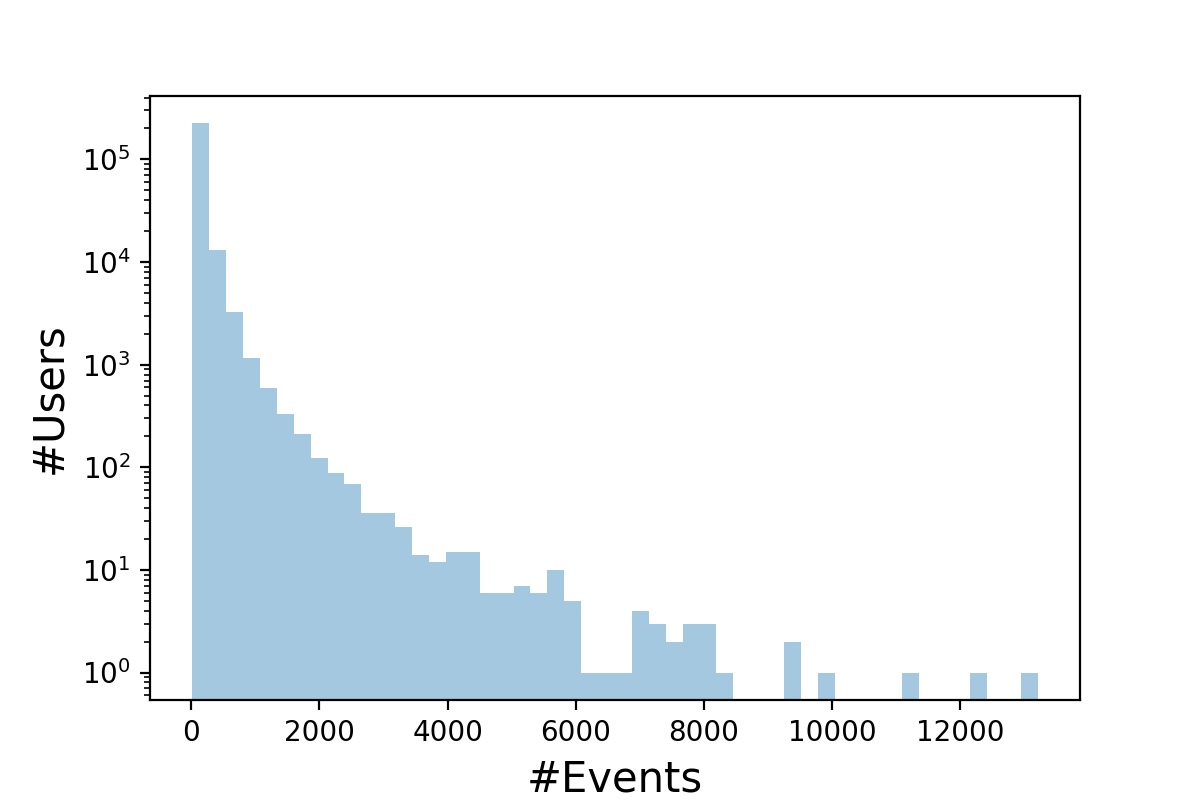
\includegraphics[width=\textwidth]{histo_user_visits.png}
    \caption{Distribution of the number of visits per user (log-scale)}
    \label{fig:histo_user_events}
\end{figure}
If we look at figure~\ref{fig:histo_user_events} we can see the distribution of the number of visits per user.
What can be seen in the histogram is a phenomenon called "The Long Tail" in the context of web analytics.
There is a very high proportion of the users which produce very little datapoints, at the same time there is a very long tail in the distribution, where some users produce extremely many events.
Thus the information that can be extracted from the majority of users is rather limited.
Of the approximately 250K users there are about 170K users that produced at most 100 events in total across all sessions.
This would explain the limited amount of cross session information we can learn when adding the user-level GRU.
Because of that the user embedding will not change much from its initial random intitialization, effectively changing nothing about the model, since without the user layer a session would be initialized at random as well.
\par
The second thing is that the product embedding greatly worsens the results in the offline as well as the online setting.
The reason for this is similar as explained above.
\begin{figure}[t]
	\centering
	\captionsetup{width=0.8\textwidth}
    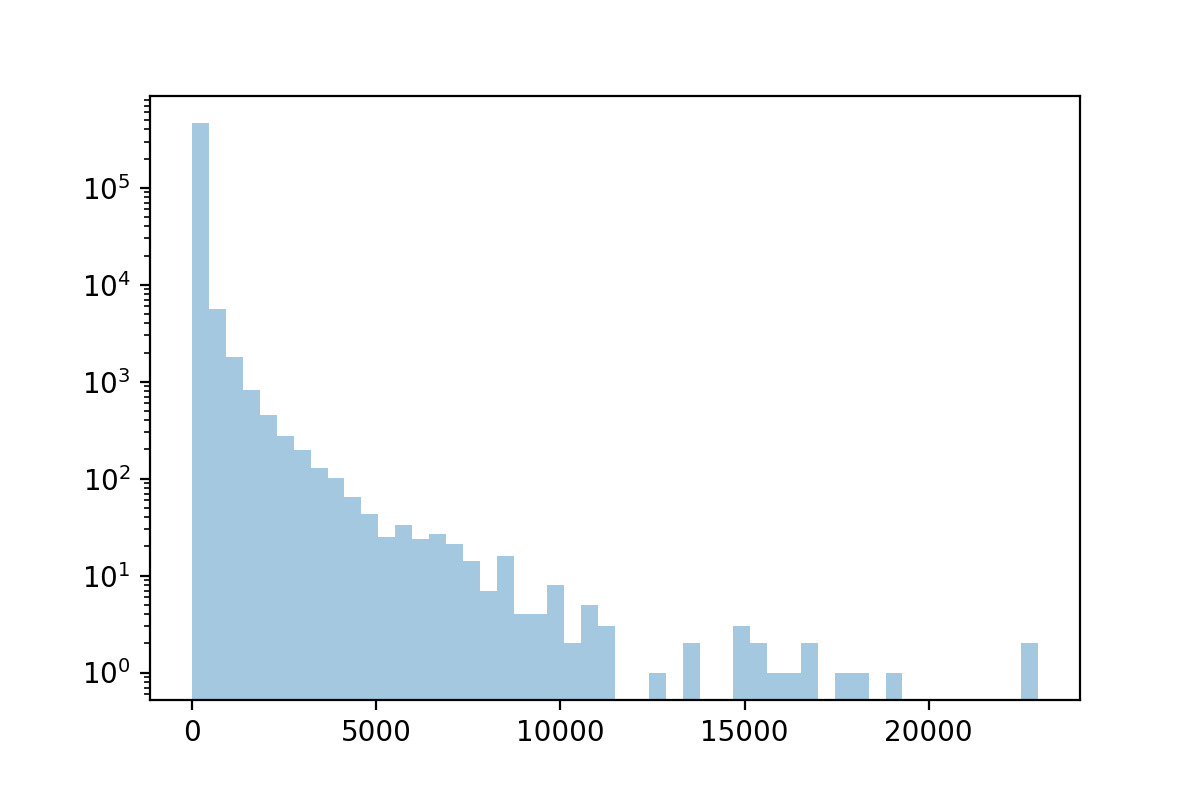
\includegraphics[width=\textwidth]{histo_product_visits.png}
    \caption{Distribution of the number of visits per product (log-scale)}
    \label{fig:histo_product_events}
\end{figure}
In figure~\ref{fig:histo_product_events} we can see the same long tail effect as with the users.
Of the approximately 470K products about 320K have at most 100 events recorded.
\begin{figure}[t]
	\centering
	\captionsetup{width=0.8\textwidth}
    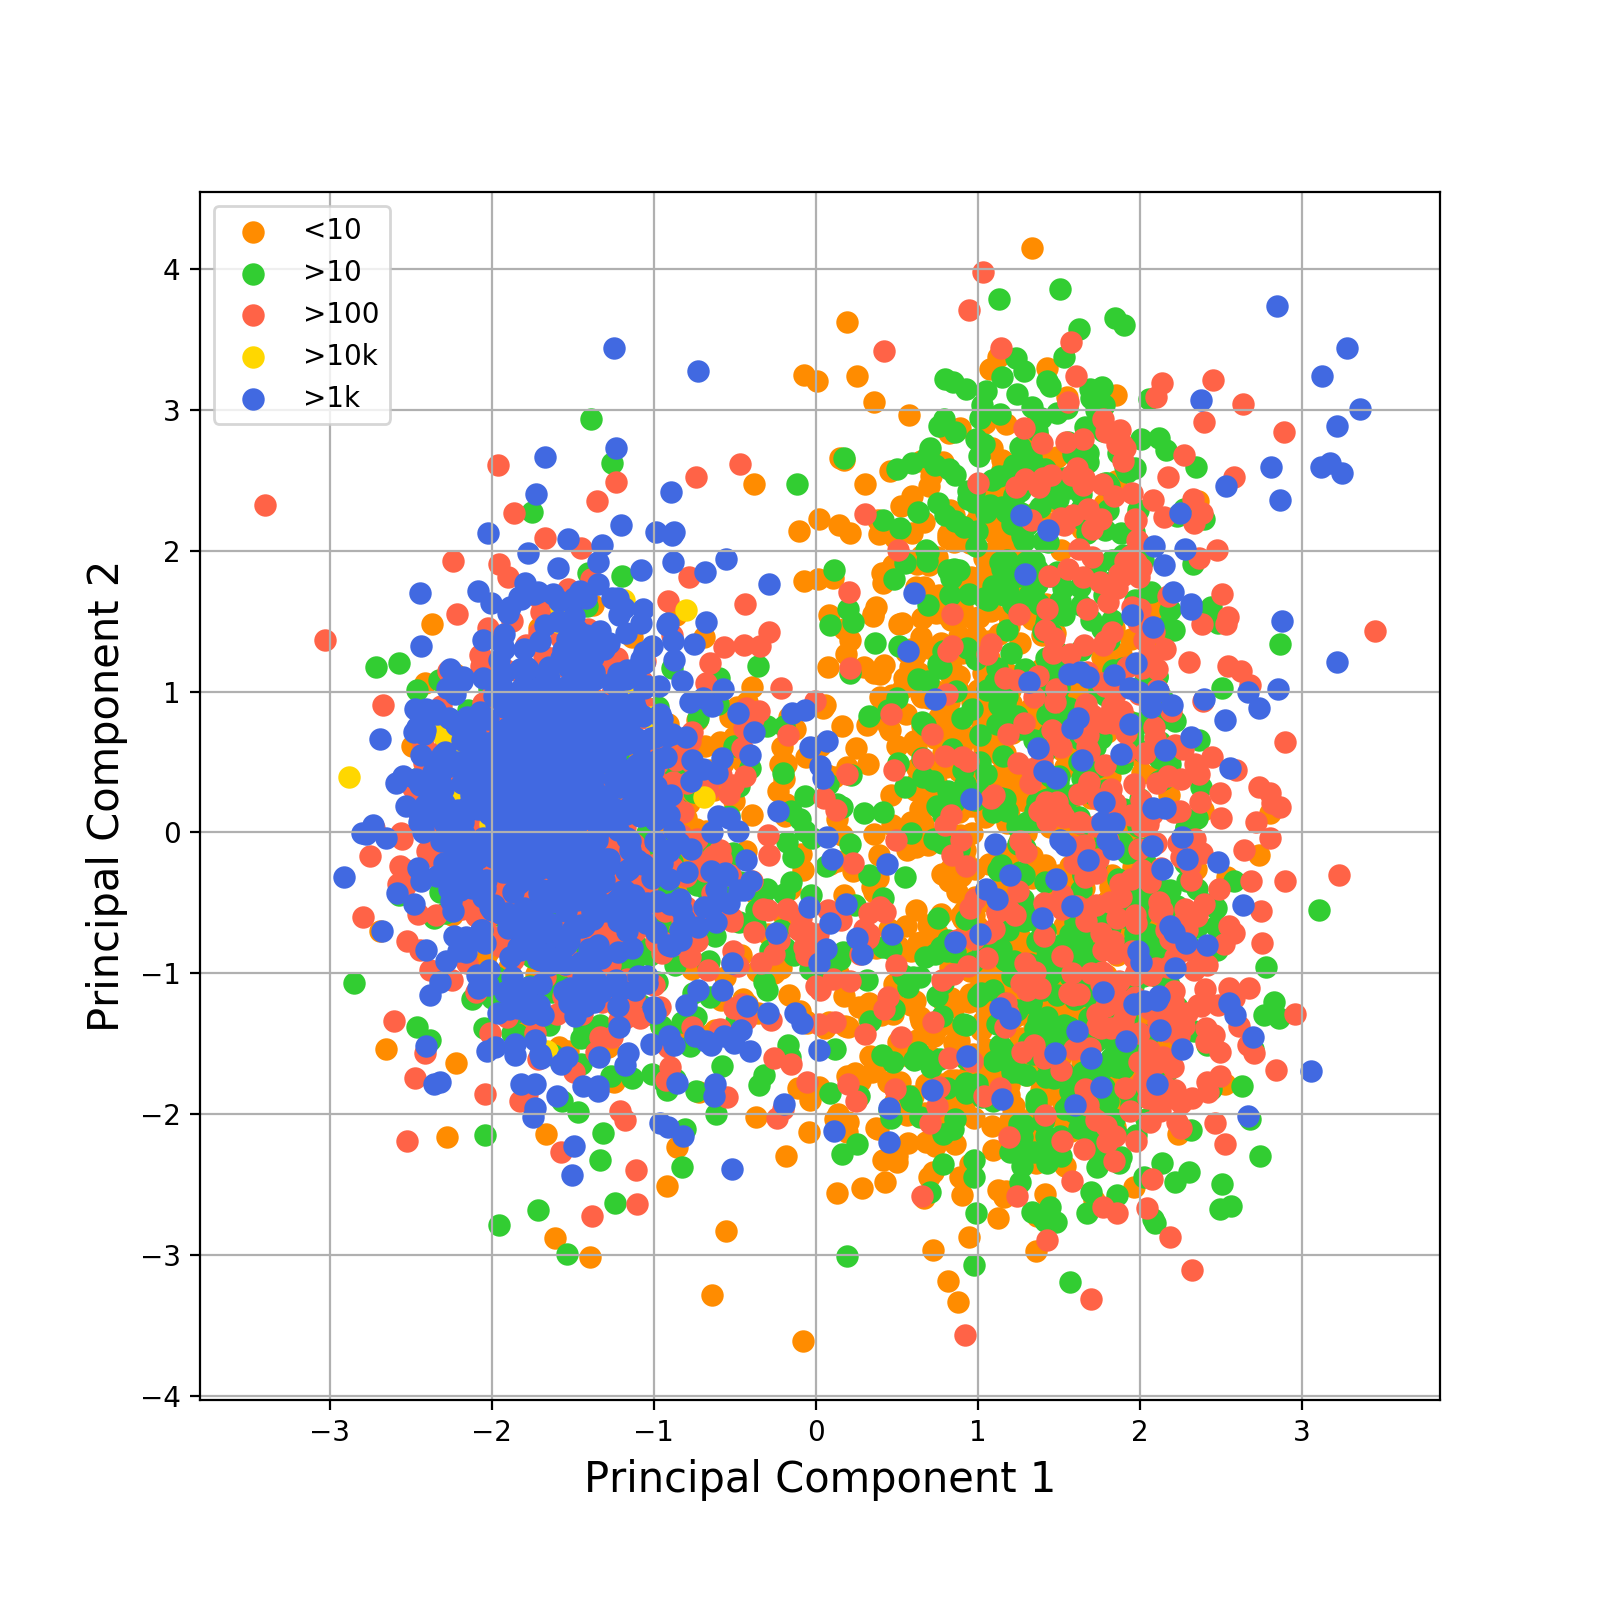
\includegraphics[width=\textwidth]{products_pca.png}
    \caption{PCA of product embeddings}
    \label{fig:products_pca}
\end{figure}
In figure~\ref{fig:products_pca} we can see a PCA analysis of the product embeddings.
As can be seen in the PCA there is a separation of datapoints in the first principal component.
\begin{figure}[t]
	\centering
	\captionsetup{width=0.8\textwidth}
    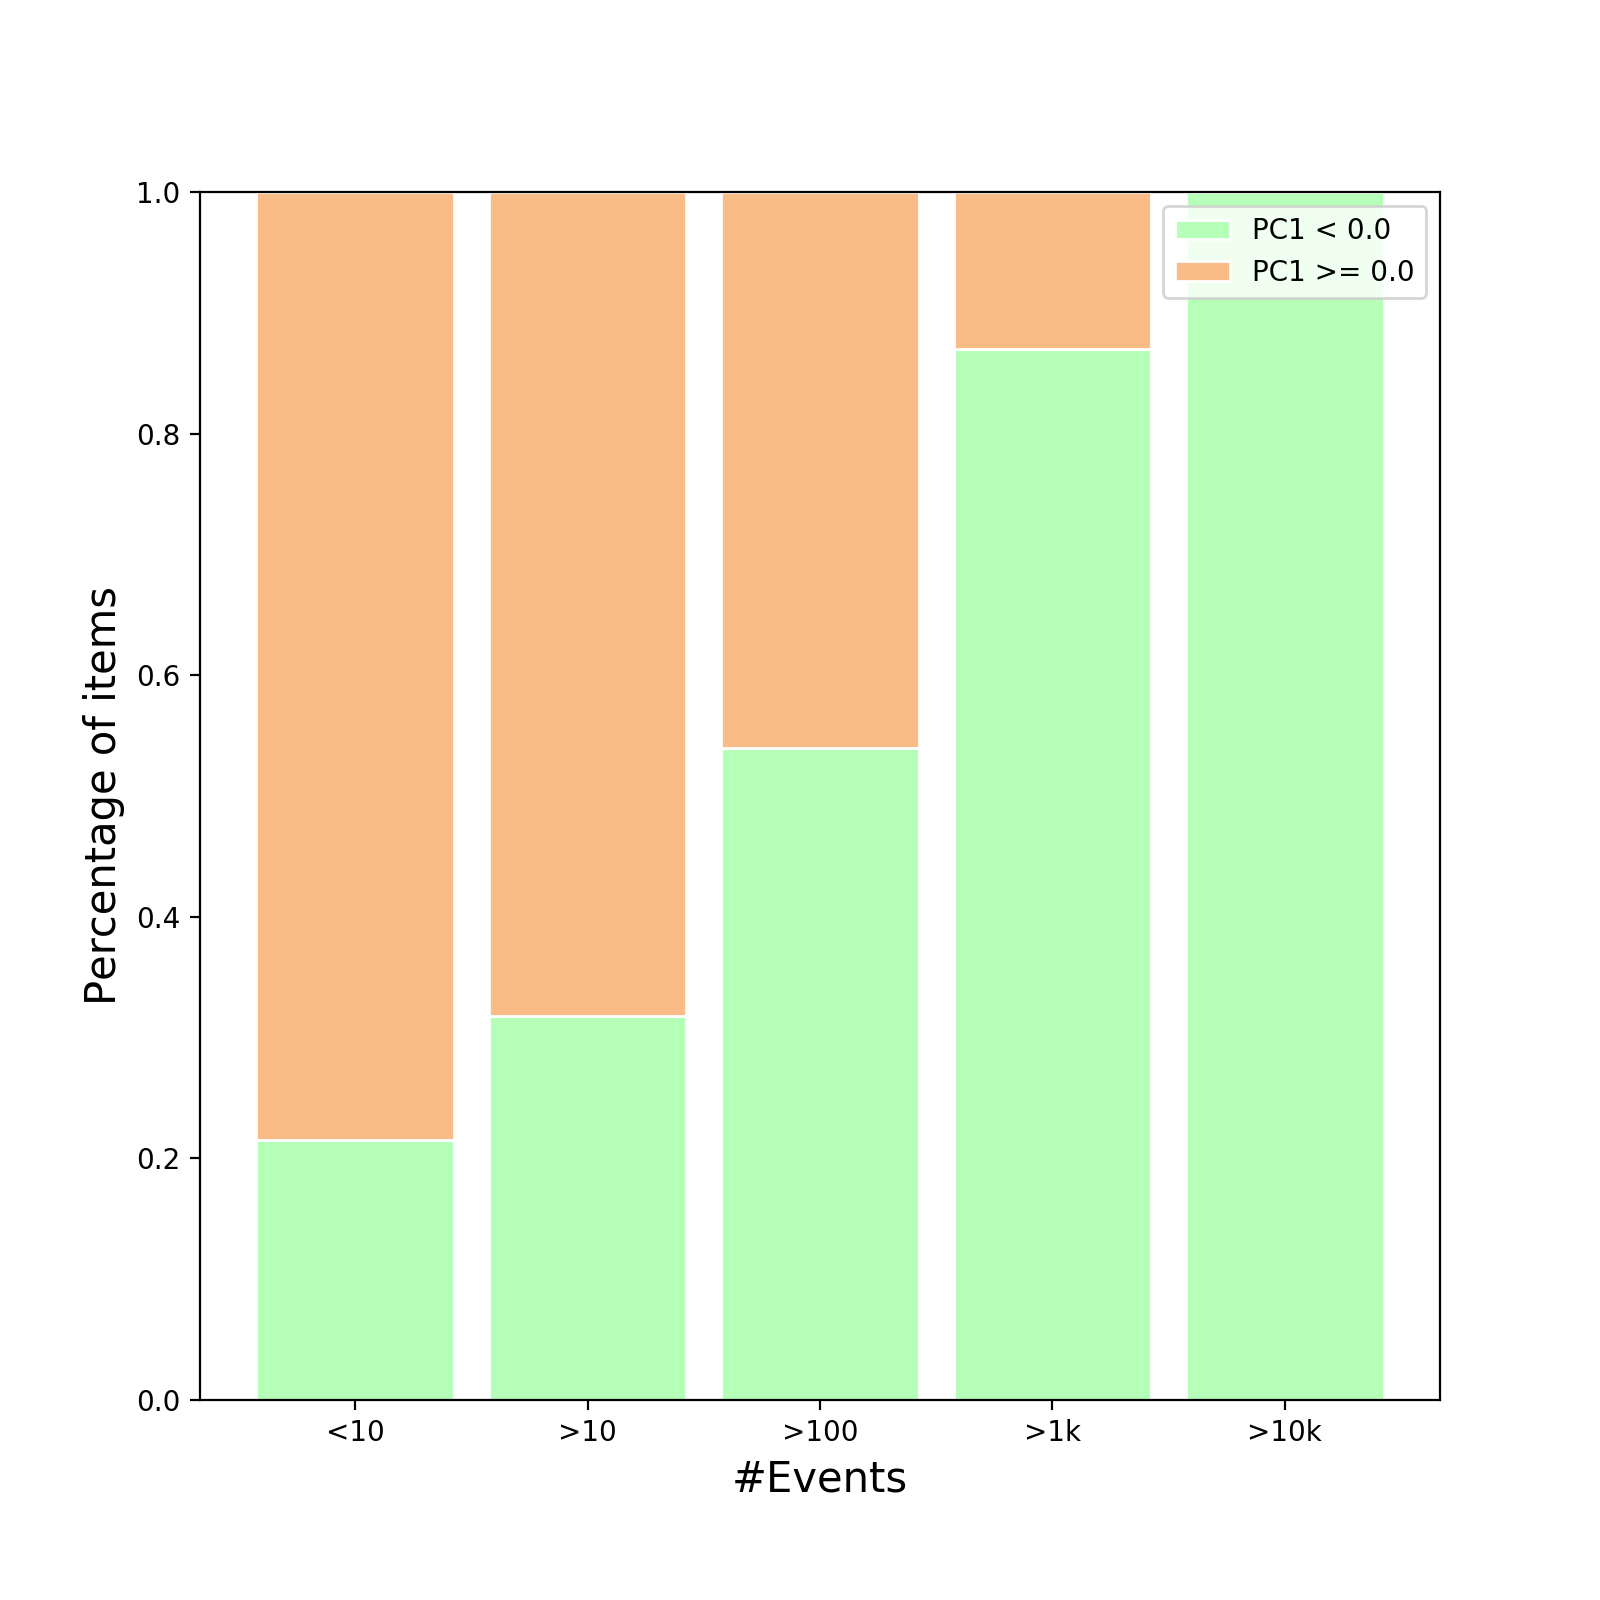
\includegraphics[width=\textwidth]{products_pca_groups.png}
    \caption{Value of PC1}
    \label{fig:products_pca_groups}
\end{figure}
In figure~\ref{fig:products_pca_groups} we can see the percentage of datapoints that have the first principal component smaller than 0, grouped by the number of events per product.
It is clear from this that the products that generate a lot of events can clearly be separated from the ones producing few events.
That means again that the majority of the product embeddings does not move much from the initial random initialization.
Therefore it can happen that for example a dining table with very few visits is very similar to a shoe with few visits, since both vectors are initialized uniformly at random drawing values from the same distribution.
The problem with this is the signal that is propagated to the GRU.
When using the one-hot encoding there is always a clear signal which product was the one that was viewed, with the product embedding this is not the case.
Therefore the network in many cases, basically receives random noise as an input, not being able to produce something else in the output layer.
This has the effect that the predictions in the models using the product embeddings are almost always the same, recommending items that are viewed many times, but do not have much relation to the currently active item.
\par
In conclusion it can be said that the sesssion-based approach clearly works, even if it does not match the performance of a commercial product, it performs better than more classical approaches to recommendation.
However personalizing these recommendations turns out to be more difficult than initially thought.
It greatly depends on the number of events produced by each user.
Therefore it might make sense to focus on personalizing the experience for the subset of users that actually produce enough events.
The same can be said for the introduction of product embeddings, the product embeddings have to be very good such that the network can interpret the signal correctly.
At least the properties of the dataset have a very large influence on the success of both the personalization of the recommendations as well as the usage of product embeddings.
\par
A future improvement of this work would be the use of transfer learning.
If the currently active item is an item with very few events, a similar item with more events can be used as a replacement as a basis for the recommendation.
However this would require a secondary similarity measure.
It would also be useful to improve the product embedding, in~\cite{content2vec} a model is introduced which, in addition to meta information also takes into account images of a product and its textual description.
Another approach to improving the product embedding could be to parametrize the distribution for the initialization of the vectors to some side-information.
This would at least remove the issue that very dissimilar products have close embeddings.
Finally another improvement that could be explored is to not only model the sequence of product detail pages, but all the different types of pages in such an online-store.
This would give the system the ability to recommend review articles or categories for the user to explore.